\chapter{Metric Relaxation}
\label{chapter:metricRelaxation}
In the previous chapters, the means of algorithm ranking have been discussed. Lots of effort has been dedicated to design algorithms that produce metrics on the dataset space induced by the attribute assignment. These algorithms were derived from the weighted $p$-norms on the attribute space. This enabled us to optimize the weights using evolutionary algorithms. We have also proven the effectivity of such approach. On the other hand, we could argue that more complex distance measure can be build on the attribute space. For instance, it seems like a good idea to enable the model to ask questions whether the attribute contain only integers or also continuous values. But instead of weighting difference of zeroes and ones, it would be perhaps a better idea to split the distance computation based on these values. For such elaborate decision, a more expressive language will be required than just a fixed-size vector of real numbers. With such added complexity we can however lose the guarantee of the attribute metric. We begin this chapter of defining relaxed versions of metrics. \emph{Semimetric} and \emph{quasimetric} are derived from metric by omitting one of the axioms -- triangle inequality and symmetry axiom respectively. We discuss which metric axioms are more important when defining a distance measure. We present a simple way of modifying arbitrary distance measure to be at least a semimetric. Then we revisit the theorems about preservations of metric from the space of attribute to the space of datasets when using attribute alignment, and we will show that the same facts hold for the preservation of semimetric. We then define a class of algorithms derived from Genetic Algorithms (see Section \ref{section:geneticAlgorithms}) called \emph{Genetic Programming} (GP). Genetic Programming, compared to the Genetic Algorithms, tries to evolve a function (or program) solving the problem instead of finding a solution to an instance of problem. Genetic Programming algorithms can be configured to produce the functions of arbitrary expression power, which will be suitable for finding more delicate attribute distance measures. We also show examples of typical GP operators. We review one of the phenomenon sometimes observable in the GP experiments -- the \emph{bloat problem}. Bloat is the tendency of some GP functions to grow in complexity, which is often accompanied by the decrease in generalization abilities of the evolved programs. In the rest of the section, we propose new batch of experiments. We discuss their expressive abilities and set their parameters in alignment with our theoretical results. We review the results of the new algorithms compared to the previous ones.

\section{Metric Spaces Revisited}
\label{section:semimetricRepairment}
In the definition of the metric (Definition \ref{definition:metric}), we have opted to use a redundant definition as the axiom 1 can be derived from the remaining axioms (Theorem \ref{theorem:metricaxiom1redundant}). This enables us however to relax the definition of the metric to introduce the terms semimetric and quasimetric:

\begin{definition}
	A \emph{semimetric} on a set $X$ is a function satisfying the first three axioms but not necessarily the fourth (triangle inequality).
	\begin{equation}
	d : X \times X \rightarrow [0,\infty),
	\end{equation}
	and for all x, y, z in X, the following conditions are satisfied:
	\begin{enumerate}
		\item $d(x,y) \geq 0$ (non-negativity).
		\item $d(x,y) = 0 \Leftrightarrow x = y$ (coincidence axiom).
		\item $d(x,y) = d(y,x)$ (symmetry).
	\end{enumerate}	
\end{definition}
\begin{definition}
	A \emph{quasimetric} on a set $X$ is a function satisfying all axioms except symmetry.
	\begin{equation}
	d : X \times X \rightarrow [0,\infty),
	\end{equation}
	and for all x, y, z in X, the following conditions are satisfied:
	\begin{enumerate}
		\item $d(x,y) \geq 0$ (non-negativity).
		\item $d(x,y) = 0 \Leftrightarrow x = y$ (coincidence axiom).
		\item $d(x,z) \leq d(x,y) + d(y,z)$ (triangle inequality).
	\end{enumerate}	
\end{definition}
In both quasimetrics and semimetrics, it is no longer possible to derive non-negativity axiom using the rest of the axioms. This is the reason why we explicitly included the first axiom into the metric definition. 

There has been a long debate in the community whether all these properties are equally important
for the similarity function in metalearning. For example, there are arguments
against the triangle inequality \cite{Ashby88towarda}, a popular example is as
follows: ``a man is similar to a centaur, the centaur is similar to a horse, but the man is completely dissimilar to the horse''. This example clearly violates the triangle inequality and speaks against using it. Moreover, it seems the coincidence axiom is also not very important. We can for example imagine, that the algorithm decides, that some of the metadata are not important for the similarity, thus returning zero even in cases where these values are different. We have addressed this by treating the attributes with the weight of zero as a noise. 
Regarding the symmetry axioms, there are some examples from the real world that are against it. For example, if we would go from place A to place B, the distance could be different from going back as we could go uphill, some paths could be blocked in one direction, etc. However, in the case of datasets, this example is not very useful because distance in the sense of dataset rather means dissimilarity than actual distance. When comparing two objects, we do not mind whether the comparison is made in a different order. Therefore, we did not consider quasimetrics further in the thesis.

Given an arbitrary distance measure $d$ on some space, we can repair the measure in such a way that it is a semimetric. For example function $d'$ defined as follows:

\begin{equation}
\label{eq:semimetricRepairment}
f(x,y) = \frac{|f'(x,y)|+|f'(y,x)|}{2}
\end{equation}
is always non-negative and symmetric. To enforce coincidence axiom, we can easily detect equal arguments on the input and return 0 otherwise. Similarly, if the $d'$ would return 0 for a non-matching input we could return some small non-negative number $\phi$ instead. Or we could return $\epsilon + d(x,y)$, for small $\epsilon > 0$. Both approaches results in semimetric, however there is a distinction. The former approach could break triangle inequality in the case $d$ was a metric. If we found three objects $k,l, z$ such that $d(k,z) < \phi/2$, $d(z, l) < \phi/2$, we could break the triangle inequality. That would happen if the $\phi$ was returned for the tuple $k,l$ instead of 0. For the triangle inequality to hold, it must be the case that the distance $\phi = d(k,l) \le d(k,z) + d(z,l)$. But at the same time, we have $d(k,z) + d(z,l)< \frac{\phi}{2} + \frac{\phi}{2}  = \phi$ from the assumptions, which is a contradiction.
We cannot do the same argument for the latter approach, as $\epsilon$ was amended to all distances of non equal objects.

\subsection{Attribute Assignment with Relaxed Attribute Measure}
In Section \ref{section:theoreticalProperties}, we have discussed how Algorithm \ref{algo:attributeAlignmentHungarian} preserves the metric properties. It turns out that Theorems \ref{theorem:metricPreservation}, \ref{theorem:metricPreservationSuportedSpaces} and Observation \ref{theorem:metricNonRestorationSupportedSpaces} are valid also for a semimetric:
\begin{corollary}
	\label{corollary:semimetricPreservation}
	Let a, b are lists of attributes, $\attributeDistance$ is a semimetric on the space of attributes $\mathbb{A}$. Then Algorithm \ref{algo:attributeAlignmentHungarian} preserves all semimetric axioms and the resulting distance $\globalDistance$ on the dataset space $\mathbb{D}$ is a semimetric.
	\begin{proof}	
	By following the proof of Theorem \ref{theorem:metricPreservation}, as the proof does not use derivation of the first metric axioms from the others (Theorem \ref{theorem:metricaxiom1redundant}), and proof of each axiom uses only the corresponding axiom on the attribute distance to prove the preservation without the use of the rest of the axioms.
	\end{proof}
\end{corollary}

\begin{corollary}
	\label{corollary:semimetricPreservationSuportedSpaces}
	Let $\mathbb{A}$ space of attributes and $A$ its subset, $\attributeDistance$ is a semimetric on $A$, $\mathbb{D}$ space of datasets. Then $\forall D \subseteq \mathbb{D}$, E supported by $A$, Algorithm \ref{algo:attributeAlignmentHungarian} preserves all semimetric axioms and resulting distance $\globalDistance$ on $\mathbb{E}$ is a semimetric.
	\begin{proof}
	By following the proof of Corollary \ref{corollary:semimetricPreservation} as the proof does not require elements outside of $D$ and $A$ and we can replace the whole $\mathbb{D}$ by $D$ and the whole $\mathbb{A}$ by $A$ respectively.	
	\end{proof}
\end{corollary}

\begin{observation}
	\label{corollary:semimetricNonRestorationSupportedSpaces}
	Let $\mathbb{A}$ be space of attributes and $\mathbb{D}$ space of datasets. Let $D$ be a subset of $\mathbb{D}$ and $\globalDistance$ a semimetric on $D$. Let $A$ be the source of $D$ and $\attributeDistance$ be a distance measure on $A$, such that Algorithm \ref{algo:attributeAlignmentHungarian} induces $\globalDistance$ using $\attributeDistance$. Then $\attributeDistance$ is not necessarily a semimetric on $A$.
	\begin{proof}
	By following the proof of Observation \ref{theorem:metricNonRestorationSupportedSpaces}, where we have shown that even though dataset distance $\globalDistance$ is a metric (thus consequently semimetric), we can define attribute distance $\attributeDistance$ to violate non-negativity.	
	\end{proof}
\end{observation}
We can draw the similar conclusions as with metric spaces. If we have a choice of optimizing between semimetric on attribute level and semimetric on dataset level, choosing the former implies optimizing the latter. This is not valid in the opposite direction.

\section{Genetic Programming}
\label{section:geneticProgramming}
To create more elaborate distance measures, more expressive language than the one used in the previous sections is required. We will also need a tool that can search in the language space and can find expressions that give a good similarity for the ranking prediction.
\emph{Genetic programming} (GP) can provide the needed functionality.

 Genetic programming is based on the same idea as genetic algorithms, where the encoding is often linear and of a fixed-length, but the search space is different. Genetic algorithms search the space of possible solutions to the problem, while genetic programming algorithms search the space of functions or programs (hopefully able to solve the problem) instead. 
 There are many ways of representing a program. Three common ways of representation used in genetic programming are \cite{FieldGuideToGeneticProgramming}:
 \begin{itemize}
 	\item \emph{Tree representation}: tree representation is traditional in genetic programming, and we will also use this representation in this thesis. Inner nodes of the tree represent operators (number of successors of the node equals arity of the operator) and leaves represent operands. Tree structures can be easily evaluated and are easy to interpret. Genetic operators are also easy to implement, as we will see later in this chapter. Usual assumption of tree representation is the property called \emph{closure} \cite{FieldGuideToGeneticProgramming}. It says that every inner node should handle arbitrary input from other operators and operands. The closure is usually obtained by using auto-conversion and/or defining operands of the same type and furthermore, every operator takes input of that type and return the output of that type. This is called type consistency. Finally, the faulty values for some operator can be handled by returning a default value for faulty input, extending the domain of that operator or decrease the fitness if the exception is thrown.
 	
 	\item \emph{Linear representation}: programs are represented as a sequence of some programming language. As we are interested in more in the actual functions taking two attribute metafeatures and not in elaborate functions taking lists or other more complex structures, Linear representation will not be considered further in this thesis.
 	
 	\item \emph{Strongly typed Genetic Programming}: proposed in \cite{typedGp}. It removes the closure requirements by defining types. This is done by introducing some restrictions into the process. We gain more freedom in defining functions. Furthermore, it can reduce the search space, as the algorithm can avoid generating some invalid input.
 	
 \end{itemize}
 The search space is determined by a language $L$ consisting of two sets – the \emph{function set} (having arity greater than zero) and the \emph{terminal set} (having zero arity). Terminals are either constants or input variables, and they occur only in the leaves of the tree representing the program. Functions are aggregating other functions and terminals, and they occur only in the inner nodes of the tree. The choice of $L$ is very important. Program solving the problem have to be encodable in this language - on the other hand, a too complex language will increase the search space exponentially, thus making finding a sufficiently good program nearly impossible. Genetic programming was used successfully in many domains. 
 
 \subsection{Initialization}
 At the beginning of the GP run, each individual in the initial population has to be randomly initialized. This can be achieved using following methods:
 
 \begin{itemize}
 	\item \emph{Full} method: This method receives an integer specifying the depth of a new individual as an input. This method creates layers sequentially. If the depth of the layer is lower than the target depth, new nodes are created by using functions, otherwise only terminals are used. This method creates a full tree of the target depth.
 	\item \emph{Grow} method: This method takes an integer specifying maximum depth as an input. New layers are created by using both functions and terminals at random. If maximum depth were to be violated, only terminals are used. By allowing terminals in the inner nodes, the distance between the root node and lists may be less than the specified maximum depth.
 	\item \emph{Ramped half-and-half}: This method creates half of the new individuals by using the full method and the other half by using the grow method.
 \end{itemize}
 
 When generating subtrees, we have to worry only about arity and generate required number of arguments. Because of the closure property we can use arbitrary inputs for every operator.
 
 \subsection{Crossover}
 The principle of the crossover operator is the same as in the original genetic algorithms.  Given two parents, one node from each parent is randomly selected. Subtrees corresponding to these nodes are swapped afterwards. This is a valid operation because of the closure property. The whole process is illustrated in Figure \ref{fig:gpcrossover}. Crossover points does not have to be selected with uniform probability. Typical GP primitive sets lead to trees with an average branching factor (the number of children of each node) of at least two, therefore  the majority of the nodes will be leaves. Consequently, the uniform selection of crossover points leads to crossover operations frequently exchanging only very small amounts of genetic material (i.e., small subtrees); many crossovers may in fact reduce to simply swapping two leaves. To counter this, authors in \cite{KozaGP} suggested the widely used approach of choosing functions 90\% of the time and leaves nodes 10\% of the time.
 
 \begin{figure}
 	\includegraphics[width=14cm]{Images/gpcrossover.png}
 	\centering
 	\caption{Example of the crossover in the Genetic Programming with the tree representation.}
 	\label{fig:gpcrossover}	
 \end{figure}
 
 \subsection{Mutation}
 Mutation alters part of the tree. A node in the parent is randomly selected. A random tree is initialized by one of the initialization method and the selected node is replaced by the new tree. Again, the closure property guarantees this to be a valid operation. The whole process is illustrated in Figure \ref{fig:gpmutation}. 
 
 \begin{figure}
 	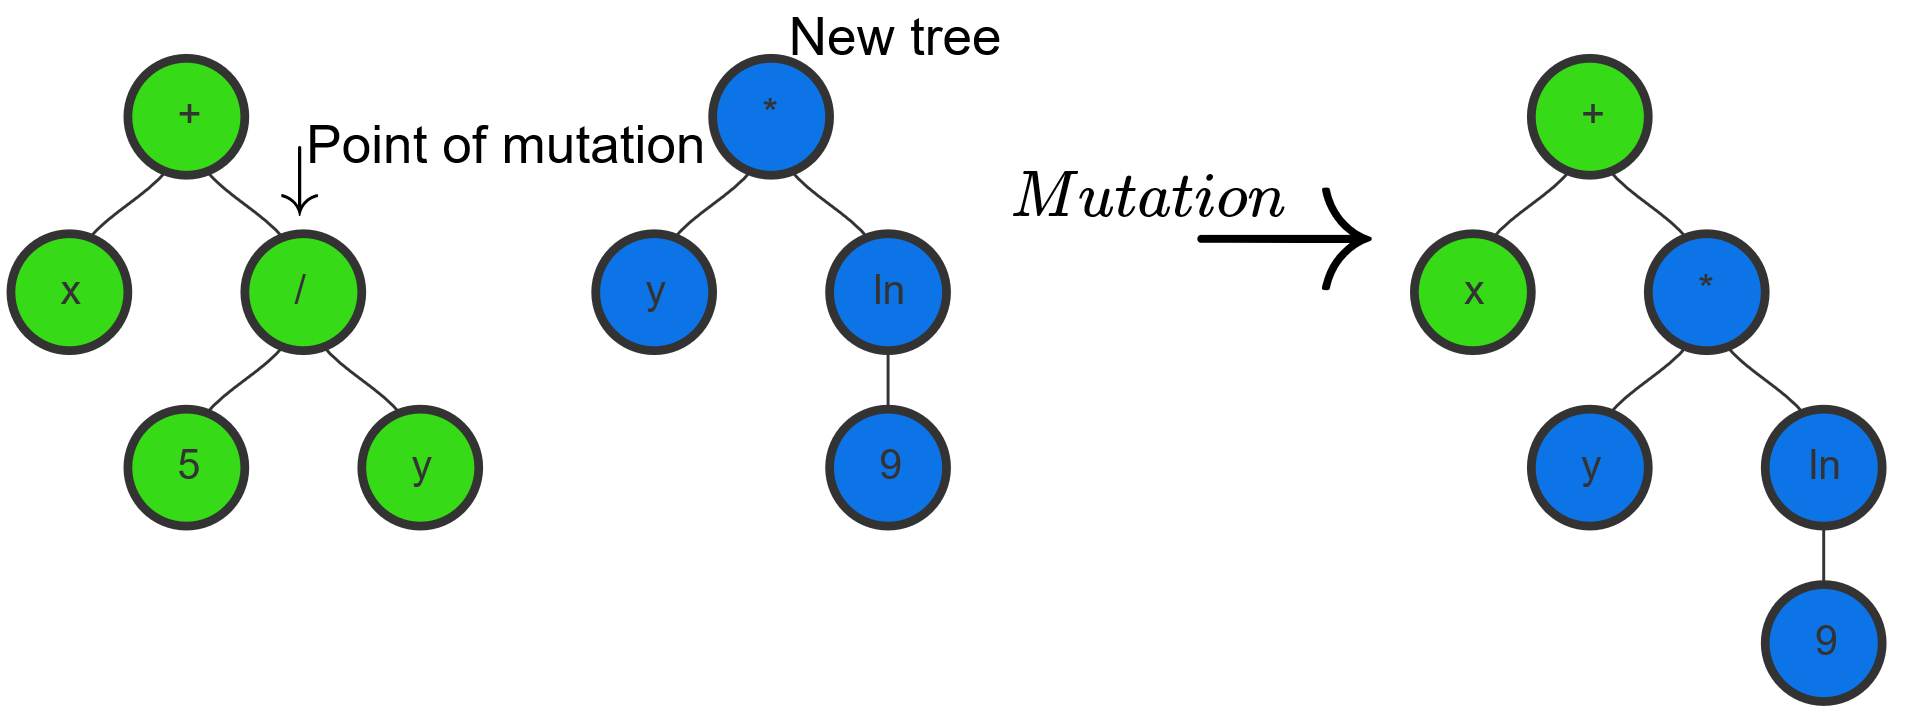
\includegraphics[width=12cm]{Images/gpmutation.png}
 	\centering
 	\caption{Example of the mutation in the Genetic Programming with the tree representation.}
 	\label{fig:gpmutation}	
 \end{figure}
 
 \subsection{Bloat Problem}
 \emph{Bloat} refers to a rapid growth of individual sizes without corresponding significant increase of fitness in later generations. In general, software bloat means that a computer program contains features that are never or rarely used. Growth alone could be beneficial, after all we are often searching complex program spaces, but without the fitness improvement it is nearly always bad. Larger individuals take more time to evaluate, take more space to store, are harder to interpret, and their ability to generalize is greatly reduced.
 There are three main theories explaining bloat \cite{FieldGuideToGeneticProgramming}:
 \begin{enumerate}
 	\item \emph{Replication accuracy theory} states that the success of a GP individual depends on its ability to have offspring that are functionally similar to the parent. As a consequence, GP evolves towards (bloated) representations that increase replication accuracy.
 	\item \emph{Removal bias theory} divides nodes in a GP tree into two categories – active code and inactive code. Inactive code is either not executed, or it is executed and its output is then discarded (for example, an inactive code would be a subtree consisting of $+(0+0+0+0)$). All remaining code is considered active. The theory observes that inactive code in a GP tree tends to be low in the tree, residing, therefore, in smaller-than-average-size subtrees. Crossover events excising inactive subtrees produce offspring with the same fitness as their parents. On average, the inserted subtree is bigger than the excised one, thus such offspring are bigger than average while retaining the fitness of their parent leading ultimately to growth in the average program size.
 	\item The \emph{nature of the program search spaces theory} predicts that above a certain size, the distribution of fitness does not vary with size. Since there are more long programs, the number of long programs of a given fitness is greater than the number of short programs of the same fitness. Over a time GP samples longer and longer programs simply because there are more of them.
 \end{enumerate}
 Techniques were designed to prevent or decrease bloat. More comprehensive survey is in \cite{LukeAntiBloatSurvey}, we will list some of the approaches:
 \begin{enumerate}
 	\item Size and depth limits. This approach checks after applying genetic operator whether the offspring is beyond the size or depth limit. If it is not, the offspring enters the population. If, instead, the offspring exceeds the limit, one of the parents is returned. Obviously, this implementation does not allow programs to grow too large. However, there is a serious problem with this way of applying size limits, or more generally, constraints to programs: parent programs that are more likely to violate a constraint will tend to be copied (unaltered) more often than programs that do not. That is, the population will tend to be filled up with programs that nearly infringe the constraint, which is typically not what is desired. The problem can be fixed by not returning parents if the offspring violates a constraint. This can be realized using two different strategies. Firstly, we can just return the oversized offspring, and assign it a fitness of 0, so that the selection will get rid of it in the next generation. Secondly, we can simply declare the genetic operation failed, and try again. This can be done in two alternative ways: a) the same parent or parents are used again, but new mutation or crossover points are randomly chosen (which can be done up to a certain number of times before giving up on those parents), or b) new parents are selected and the genetic operation is attempted again.
 	\item Anti-Bloat genetic operators. This approach modifies genetic operators to reduce the bloat. Among the bloat-control methods are size fair crossover and size fair mutation \cite{langdonSizeFairCrossover}. These work by constraining the choices made during the execution of a genetic operation so as to actively prevent growth. In size-fair crossover, for example, the crossover point in the first parent is selected randomly, as in standard crossover. Then the size of the subtree to be excised is calculated. This is used to constrain the choice of the second crossover point so as to guarantee that the subtree chosen from the second parent will not be “unfairly” big.
 	\item Anti-Bloat selection modifies the selection so that bloated individuals have lower probability to be selected into next generation. Tarpeian method \cite{PoliAntiBloatTheoreticallyMotivated} controls bloat by acting directly on the selection probabilities in the following equation:
 	\begin{equation}
 	E[\mu(t+1)-\mu(t)]=\sum_{t}l(p(l,t)-\phi(l,t)),
 	\end{equation}
 	where $E$ is the expectation operator, $\mu(t+1)$ is the mean size of the programs in the population at generation $t+1$, $l$ is the program size, $p(l,t)$ is the probability of selecting programs of size $l$ from the population in generation t and $\phi(l,t)$ is the proportion of programs of size $l$ in generation $t$. This is done by setting the fitness of randomly chosen longer-than-average programs to 0. This prevents them from being parents. By changing how frequently this is done, the anti-bloat intensity of Tarpeian control can be modulated. An advantage of the method is that the programs whose fitness is zeroed are never executed, thereby speeding up runs. Parsimony pressure method \cite{KozaGP} changes the selection probabilities by subtracting a value based on the size of each program from its fitness. Clearly, bigger programs have lower fitness and potentially less offspring under this approach. That is, the new fitness function is:
 	$f_{new}(x)  = f(x)-c l(x)$, 
 	where $l(x)$  is the size of program $x$, $f(x)$ is its original fitness and $c$ is a constant known as the parsimony coefficient.
 \end{enumerate} 
 
 \section{Experiment Proposal}
 \label{section:relaxationExperiments}
 We want to extend our whole framework with more expressive attribute distance. Again, we would like to get attribute distance in the form that can fit into our workflow. In the metric experiments we decided to use attribute alignment with selectors, as we wanted to utilize even metadata specific numerical and categorical attributes. We will do the same decision again. That gives us more specific idea for what we are looking for -- we need two functions, first computing distance between two numerical attributes and the second computing distance between two categorical attributes. In the previous section, we argued that we will use tree representation for evolved functions. To get there, we need to specify functions, terminals, make sure that we maintain the closure property, decide on the initialization and genetic operators. The main thing we need to keep in mind when proposing the whole design of the GP algorithm is that we want to generate more expressive functions. However, we will make one exception. The algorithm from Section \ref{section:firstExperiments} also evolves the weights of each selector. To evolve them using GP we would have to combine GP with GA as the vector of weights is not a tree. We decided to use the same weights for the numerical and categorical selector instead of evolving them.
 
 If not said otherwise, the proposed functions and terminals can be used regardless of the type of program evolved. All functions and terminals will be type consistent, which means that all functions will have all arguments and output of the same type. This type will be a real number in our case. If some $n$-ary function is not defined on the whole $\mathbb{R}^n$, we will propose its extended definition on the whole $\mathbb{R}^n$.
 
 \subsection{Functions}
 When discussing which function to use, we have argued that if we want to create trees with more expressive power than the previous experiments with the metric based on $p$-norms. To do that we should start by enabling the same functionality -- to add function for addition, division, square root (as we were using only $p \in \left\{1, 2, \infty  \right\}$), maximum of two values (required by the infinity norm), $p$-th power and abs. We should initialize the function set of the GP accordingly. 
 
 \begin{itemize}
 	\item Basic mathematical functions: add, subtract, multiply and divide will be used. Only division needs to be generalized. The following generalization was chosen:
 	\begin{equation*}
 	\text{Divide}(x,y)=
 	\begin{cases}
 	0; \text{ if } y = 0, \\
 	\frac{x}{y}; \text{ otherwise}.
 	\end{cases}
 	\end{equation*}
 	Based on the discussion above, we also included maximum. We decided not to include power of $p$ explicitly, as for $p=1$ or $p=2$ it can be easily evolved by the times function.
 	\item Boolean functions: normally, boolean function returns tree and false, which is usually used for branching further in the program. This would however break the closure. For the sake of type consistency, we used a trick to design Boolean functions and we proposed boolean functions (with some arity $i$) according to the following pattern:
 	\begin{equation*}
 	\text{Boolean}(a_1, \dots a_n,x,y)=
 	\begin{cases}
 	x; \text{ if } b(a_1, \dots, a_n), \\
 	y; \text{ otherwise}.
 	\end{cases}
 	\end{equation*}
 	Namely:
 	\begin{equation*}
 	\text{LessThan}(a_1,a_2,x,y)=
 	\begin{cases}
 	x; \text{ if } a_1 < a_2, \\
 	y; \text{ otherwise}.
 	\end{cases}
 	\end{equation*}
 	\begin{equation*}
 	\text{LessThanOrEqual}(a_1,a_2,x,y)=
 	\begin{cases}
 	x; \text{ if } a_1 \le a_2, \\
 	y; \text{ otherwise}.
 	\end{cases}
 	\end{equation*}
 	
 	In theory, maximum function can be obtained by these boolean functions. However, it is quite complicated to evolve as $\max(x,y)$ corresponds to $\text{LessThan}(x,y,y,x)$ and all four inputs must match. As the maximum function is quite important, we decided to add the maximum as an extra function nevertheless.
 	\item 	Other functions: we have introduced square root and base 2 logarithm. These functions were generalized by following:
 	\begin{equation*}
 	\text{SquareRoot}(x)=
 	\begin{cases}
 	\sqrt{x}; \text{ if } x \ge 0, \\
 	\sqrt{|x|}; \text{ otherwise}.
 	\end{cases}
 	\end{equation*}
 	\begin{equation*}
 	\text{Log}_2(x)=
 	\begin{cases}
 	\log_2(x); \text{ if } x \ge 0, \\
 	0; \text{ if } x = 0, \\
 	\log_2(|x|); \text{ otherwise}.
 	\end{cases}
 	\end{equation*}
 \end{itemize}
 Some other functions were also discussed:
 \begin{itemize}
 	\item Polynomial functions: We did not want to expand the domain too much, and this type of functions can be expressed by combining basic functions, so we did not introduce polynomials into population.
 	\item Periodic functions: like sin, cos. We have argued that an evolving program will not benefit from periodicity, thus we did not introduce such functions into GP domain.
 	\item Boolean functions greater than, greater than or equal. These were not introduced into the domain because they can be expressed by the means of Boolean functions already in the domain:
 	\begin{equation*}
 	\text{GreaterThan}(a_1,a_2,x,y)=\text{LessThanOrEqual}(a_2,a_1,x,y),
 	\end{equation*}
 	\begin{equation*}
 	\text{GreaterThanOrEqual}(a_1,a_2,x,y)=\text{LessThan}(a_2,a_1,x,y).
 	\end{equation*}
 \end{itemize}
 
 \subsection{Terminals}
 
 \begin{enumerate}
 	\item Constant terminals: we have proposed terminals that represent real and integer numbers. When creating such a terminal, a random number is generated and set as a value of the new terminal.
 	\item Metadata Terminals: again, we wanted to make the GP at least expressively strong enough to be able to evolve the same functions created in the previous section. In order to do this, we should cover all the attribute metadata used in the metric experiments. By the nature of metadata, some of them will be available only for the categorical trees and some for the numerical trees being evolved. Every metadata will be initialized with either one or zero. As the distance tree computes the distance function of two datasets $a$ and $b$, the zero or one will define whether the value of the terminal variable should be taken from the metadata of dataset $a$ or $b$.
 \end{enumerate}
 
 Random number terminals were also discussed. We have argued that an evolved program would not benefit from stochasticity, therefore we did not introduce such terminals into domain. Note that this is different from generating constants, because random number terminals generate a new number each time they are evaluated.
 
 The example with the individual generated for the numerical distance is in Figure \ref{fig:individualExample}.
 
 \begin{figure}
 	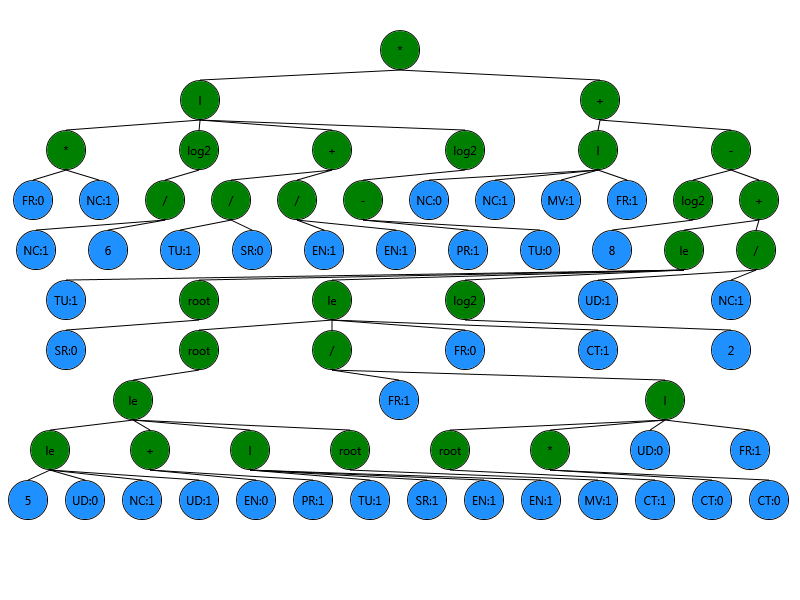
\includegraphics[width=14cm]{Images/individualExample.png}
 	\centering
 	\caption{Example of the tree evolved by the GP for the numerical distance between two attributes. The terminals are blue compared to inner-nodes which are true. The label in the node describes the type. For instance, label $l$ represents $\text{LessThan}$ function, similarly \emph{UD:0} is a variable gaining a value depending whether an attribute corresponding to the left argument (left is determined by the number 0) correspond to an uniform distribution.}
 	\label{fig:individualExample}	
 \end{figure}
 
 \subsection{Algorithm Specification}
 We need to evolve two trees. We are going to evolve these two trees as one individual. The mutation and crossover will be first applied on the categorical trees and then also on the numerical trees. As the initialization methods for the evolution, we will use the ramped half-and-half to initialize every tree. Ramped half-and-half was chosen because according to some authors \cite{FieldGuideToGeneticProgramming}, it creates more diversity. The initial maximal depth was set to 6. The mutation and crossover probabilities were set regardless of whether they are used for the categorical or numerical part of an individual. The mutation chance was set according to our previous experiments to 0.2. The probability of crossover happening was set to 0.7. The termination criterion was set to the generation count. We did not want to encourage bloating and over-fitting, so the generation target was set to 80. We believe this was the reasonable amount of generation to evolve reasonably good distance measures. Compared to the previous experiments with genetic algorithm, we also increased the population size to 120 individuals. GP is more dependent on bigger populations, as a lot of distance measures generated really bad input compared to the genetic algorithms where everything was a $p$-norm, and even the worst weights produced somewhat reasonable output.
 
 For the rest of the workflow settings, we will not make any changes. We set up number of neighbours for the $k$-NN to 17 and use the dummy attribute as the one already in the attribute space given by the median of every metafeature.
 
 Given two datasets $a$ and $b$, respectively their numerical and categorical metafeatures, the evolved tree can now compute the distance using Algorithm \ref{algo:combinedAlignmentHungarian}. This does not guarantee any of the metric properties. For instance, algorithm can produce zero easily by instantiating the minus node with two children -- each of them initiated by a constant of the same value. It would be very hard to constrain the GP algorithm to evolve only metrics or semimetrics. It would require either a limited set of functions the algorithm can use,
 or complicated operators, which would ensure these properties. Instead, based on the discussion in Section \ref{section:semimetricRepairment}, we decided to amend the values produced by the trees according to Equation \ref{eq:semimetricRepairment}, return $0$ if $x=y$ and add a small $\epsilon > 0$ if $\delta(x,y)=0$ and $x \neq y$. This will guarantee that we will have a semimetric on the attribute space.
 According to Corollary \ref{corollary:semimetricPreservation}, the resulting distance $\globalDistance$ on the dataset space is a semimetric. Thus, we sacrificed triangle inequality to gain more expressive language to describe attribute distance measures. Other option would be to repair the resulting distance between datasets. We have decided to repair the attribute distance, as aligned to the results of Corollary \ref{corollary:semimetricPreservationSuportedSpaces} and Observation \ref{corollary:semimetricNonRestorationSupportedSpaces}.
 
 The increase in the population size slightly increased the amount of time to conduct the experiments. Also, if the GP tree was deep enough, its evaluation usually took slightly more time compared to $p$-norms. This was a major factor as the function was evaluated many times. Despite this fact, we decided not to lower the number of runs so the results are easier to compare. Therefore, the number of runs was again set to 10.
 
 The whole workflow with the GP and the semimetric repairment is shown in Figure \ref{fig:BigPictureGp}.
 
 \begin{figure}
 	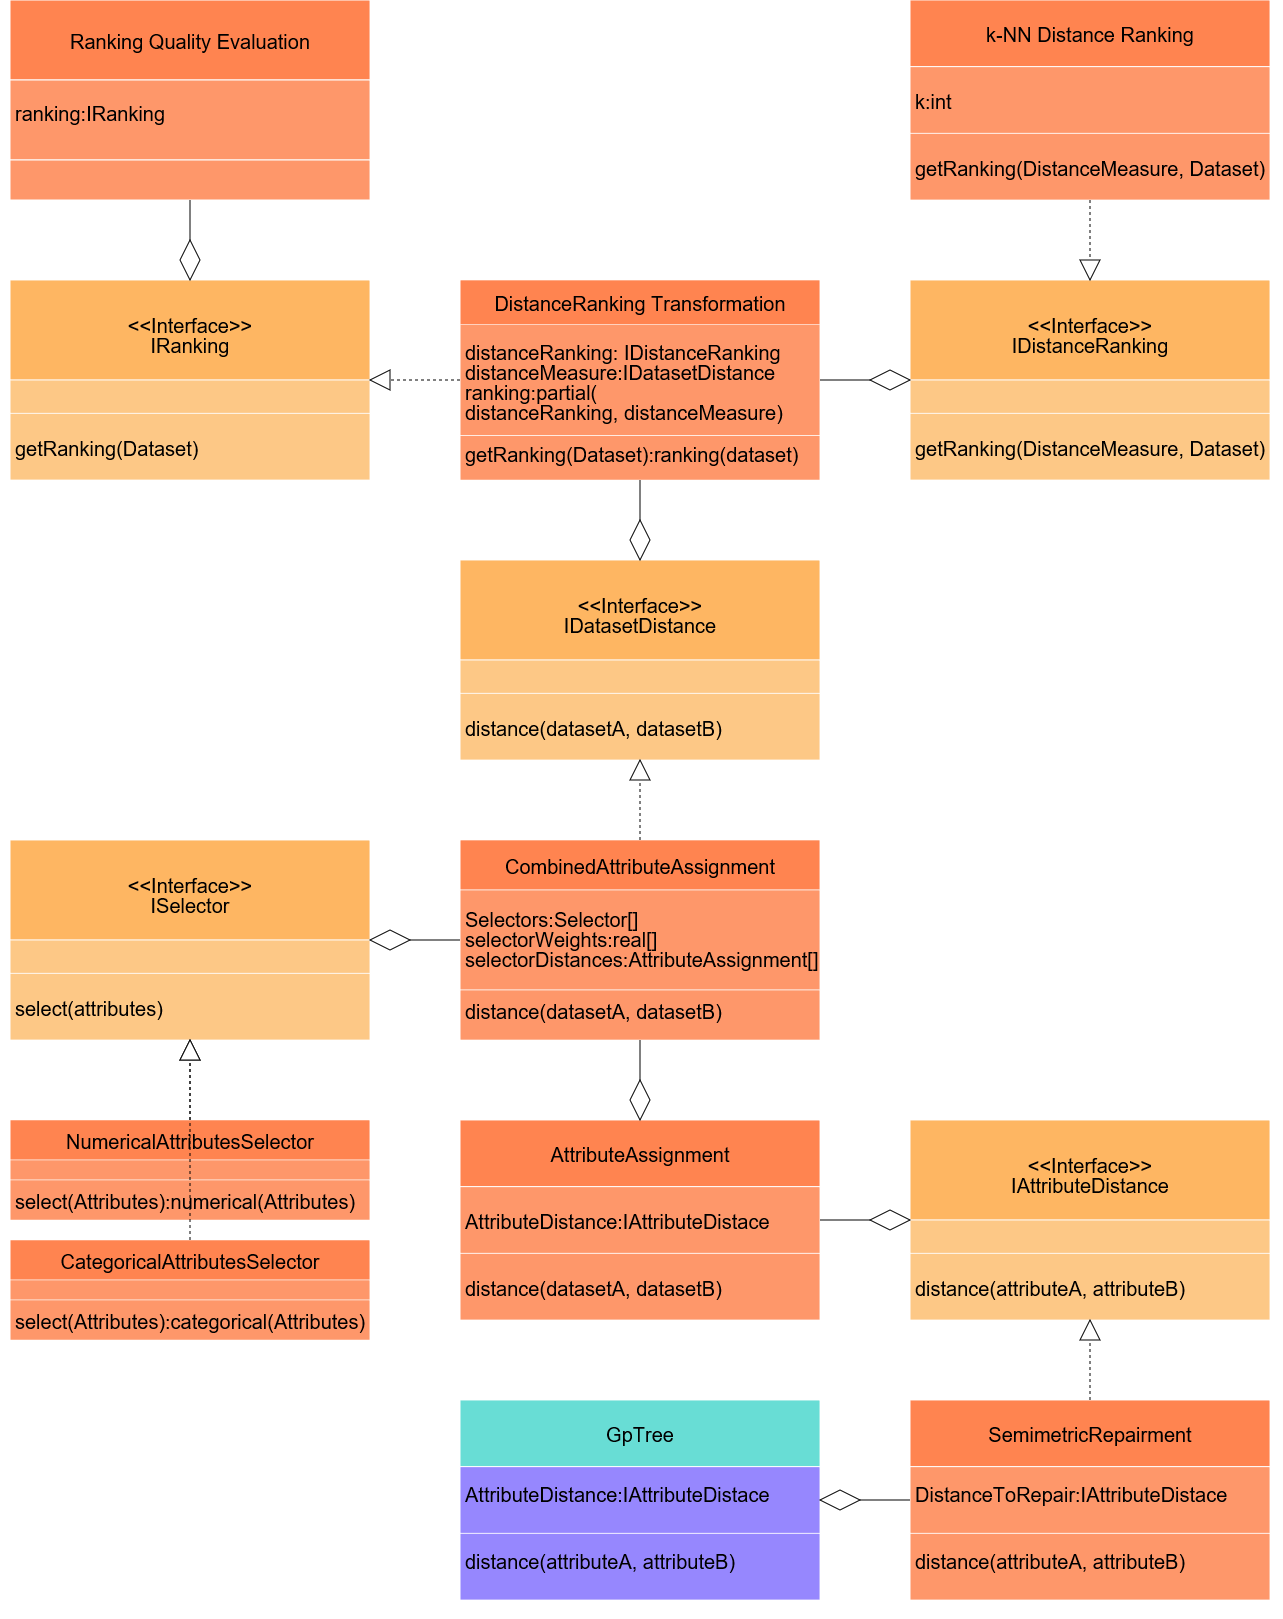
\includegraphics[width=15cm]{Images/BigPictureGp.png}
 	\centering
 	\caption{UML diagram of the workflow for the GP experiments. This time the focus will be on the GP tree, which is going to be evolved using the genetic programming by the fitness from the Ranking Quality Evaluator.}
 	\label{fig:BigPictureGp}	
 \end{figure}
 
 \subsection{Results}
 The results are shown in Table \ref{table:gpResults}. The GP managed to get above the baseline on the validation set in three out of 10 cases. It is not surprising that the statistical comparison of the GP and other algorithms shown in Table \ref{table:gpResultsComparisonWithOthers} resulted in all algorithms except the baseline outperforming the GP.
 
 These poor results could be explained by overfitting, as the training results were decent enough. For example, bloating occurred -- in the first generation the average number of nodes was around one hundred after the initialization. We could observe values above one thousand in the generation 70. This is not a rare behaviour of algorithms with high expression capabilities, as they can very easily learn some noise present in the training data. In the next chapter, we will try to improve generalization abilities of the trees being evolved.
 
 \begin{table} 
 	\caption{Evaluation of the ranking quality of the trees produced by the GP algorithm on the testing dataset.}
 	\label{table:gpResults}
 	\centering 
 	\renewcommand{\arraystretch}{1.3}
 	\begin{tabular}{c c}
 		\hline %inserts horizontal line
 		Run &  GP Result\\
 		\hline 
 			1 & 0.546221	 \\ 
 			2 &	0.542101 \\
 			3 & 0.541881 \\
 			4 & 0.540339 \\
 			5 &	0.538439 \\
 			6 & 0.536444 \\
 			7 &	0.536215 \\
 			8 & 0.532274 \\
 			9 & 0.530289 \\
 			10& 0.512501 \\
 			median & 0.537441 			 	
 	\end{tabular}
 \end{table}
 
 \begin{table}[ht]		
 	\centering
 	\caption{Statistical comparison of GP and previous algorithms and their ranking quality results on the validation set. Y stands for GP significantly worse than algorithm in the corresponding column, N stands for Not able to reject the null hypothesis (algorithms equally performing). }
 	\label{table:gpResultsComparisonWithOthers}	
 	\begin{tabular}{r|cccccccccc}
 		&
 		\rot{Aggregation, $p=1$} &
 		\rot{Aggregation, $p=2$} &
 		\rot{Global, $p=\inf$} &
 		\rot{Global, $p=1$} &
 		\rot{Global, $p=2$} &
 		\rot{Aggregation, $p=\infty$} &
 		\rot{Assignment, $p=2$} &
 		\rot{Assignment, $p=\infty$} &
 		\rot{Assignment, $p=1$} &
 		\rot{Baseline} 		
 		
 		\\ \hline
 		GP        & Y  & Y & Y & Y&Y &Y &Y &Y &Y & N  \\   		
 		\hline
 	\end{tabular} 
 \end{table}